\begin{kasten}
    \section*{ \hspace{0.1cm} {\color{red} \underline{SUMMARY}}}
    \Large{
%\hspace{6mm}We implemented Boehm-Turner's model of agile
%and plan-based software development. That tool is
%augmented with an AI search engine to find the key
%factors that predict for the success of agile or traditional 
%plan-based software developments. According
%to our simulations and AI search engine: (1) in no
%case did agile methods perform worse than plan-based
%approaches; (2) in some cases, agile performed best.
%Hence, we recommend that the default development
%practice for organizations be an agile method.

%\vspace{3mm}
%\hspace{6mm}The simplicity of this style of analysis begs the
%question: why is so much time wasted on evidence-less
%debates on software process when a simple combination of simulation 
%plus automatic search can mature
%the dialogue much faster?
%\hspace{6mm}POM2 is a software development process model. POM2 is an expansion of a previous model, POM, presented at ASE'08 by Port, Olkov, and Menzies. 
%
%\hspace{6mm}Using the 5 Boehm Turner scales, we model the size and makeup of the project requirements and personel of an individual project. Using this model, the project is completed using 2 different prioritization policies and the scored. The score is a function of the cost and value of the project. The score is used with our AI search engine, KEYS, to find the treatments that will maximize the resultant score.
%
%\hspace{6 mm}This model aims to provide emperical evidence to the agile versus plan based software development debate. With this model, a business can determine what changes to make to the project to increase the $value/cost$ ratio.
\hspace{6mm}Why is so much time wasted on evidence-less debates on
software process when a simple combination of simulation plus automatic search can mature the dialogue much
faster?

\vspace{3mm}
\hspace{6mm}Here, we implemented Boehm-Turner's model of agile and
plan-based software development. That tool is augmented
with an AI search engine to find the key factors that predict 
for the success of agile or traditional plan-based software 
developments. According to our simulations and AI
search engine: (1) in no case did agile methods perform
worse than plan-based approaches; (2) in most cases, agile performed
much better. Hence, we recommend that the default 
development practice for organizations be an agile
method.
    }
\end{kasten}

\begin{kasten}
  \section*{ \hspace{0.1cm} {\color{red} \underline{SIMULATOR STRUCTURE}}}
\large{
  \begin{minipage}{5cm}
   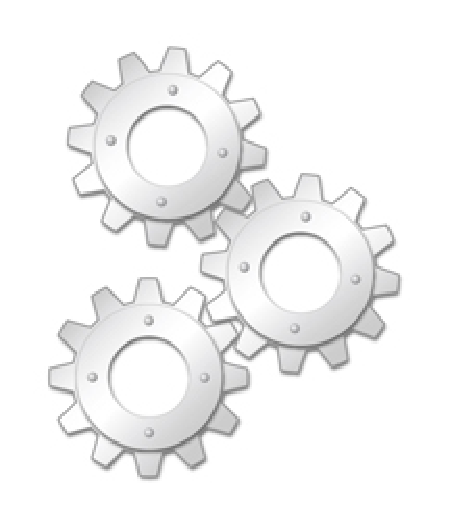
\includegraphics[width=4cm]{gear.eps}
 \end{minipage}
\begin{minipage}{8cm}
POM2 shuffles requirements through three stages: ``to-do'', ``planned'', and ``completed''.
\textit{Requirements} are represented as cost/value pairs. 
\textit{Projects} are requirements organized into acyclic trees. 
Requirement dependencies are represented by edges between nodes, with 
the constraint that all children must be completed before parents.
Requirement nodes are assigned children based on an exponential distribution: 
\begin{math} \frac{1}{X} \% \end{math} of nodes have X children.
\end{minipage} 

\vspace{3mm}
A \textit{team} contains a varying number of members. Each team is assigned a subtree from within 
the project tree, and maintains a \textit{plan} which represents the set of requirements to be completed next iteration.
The plan's size is determined by the \textit{team's budget}, and requirements in the plan are selected from 
team's project subtree. Work is completed in \textit{iterations}. A team completes a certain number of requirements 
per iteration. During each iteration, it is possible for a team to ``discover'' new requirements.  
The number of new requirements are calculated using \eq{size}: 
\begin{equation}\label{eq:size}size * 2.5\end{equation}
\textit{Inter-team cooperation} is modelled by creating dependencies between trees at the same level.
All requirements in a team's plan are ordered by a \textit{prioritization policy}. 
A project is completed when all subtrees are completed or management orders early termination

}
\end{kasten}

\begin{kasten}
    \section*{ \hspace{0.1cm} {\color{red} \underline{PRIORITIZATION POLICIES}}}
    \large{
A prioritization policy determines how many requirements are initially known and
how the plan is modified when new requirements arrive.

\vspace{3 mm}
POM 2 explores two prioritization policies:
\begin{smallenum}
\item Plan Based (PB) : A non-agile development method
  where requirements are sorted once at the start of development
  using the original \(\frac{value}{cost}\) numbers assumed at the start 
  of the project.
\item Agile2 (AG2) : A development method where requirements are sorted every iteration on  policies sort requirements (every iteration) on \(\frac{value}{cost}\). 
\end{smallenum}
\vspace{-0.2em}
}
\end{kasten}
